\chapter{Arhitektura i dizajn sustava}

		Arhitektura programske potpore predstavlja strukturu sustava ili više njih koje sadrži elemente, njihova obilježja i odnose među njima. Temeljni razlozi definiranja arhitekture:		

	\begin{itemize}
		\item 	{poboljšava razumljivost i komunikaciju sudionika}
		\item 	{pomaže u donošenju temeljnih odluka pri izradi projekta}
		\item 	{omogućava rano uočavanje pogrešaka u oblikovanju}		
		\item         {moguće ponovno korištenje rješenja (engl. reuse)}
	\end{itemize}

	U konačnici, efikasno strukturiranje arhitekture programske potpore dovest će do poboljšanja kvalitete finalnog produkta projekta.

	\vspace{10mm} %10mm vertical space

	Koristimo objektno usmjerenu arhitekturu koja najbolje odgovara razvoju složene web aplikacije namijenjene za što više korisnika u stvarnom vremenu. Možemo ju klasificirati na četiri ključna dijela koji osiguravaju izvršavanje naredbi korisnika: 
		
	\begin{packed_enum}
		\item 	{Web preglednik}
		\item 	{Web poslužitelj}
		\item 	{Web aplikacija}
		\item 	{Baza podataka}
	\end{packed_enum}			

		\begin{figure}[H]
					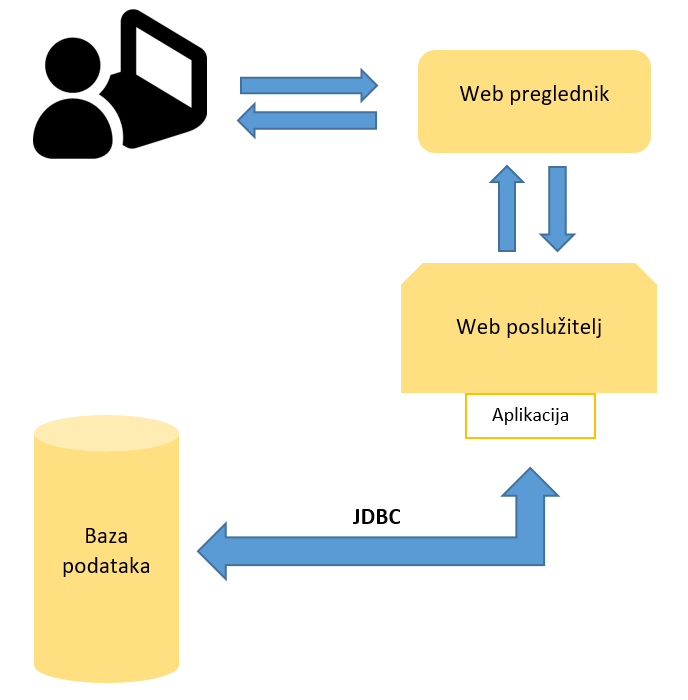
\includegraphics[scale=0.8]{arhitektura/arhitektura_sustava.png} %veličina slike u odnosu na originalnu datoteku i pozicija slike
					\centering
					\caption{Arhitektura sustava}
					\label{fig:arhitektura}
		\end{figure}

	\vspace{5mm} %5mm vertical space

		Web aplikacija će se temeljiti na modelu klijent-poslužitelj, što je danas i najčešće korišteni model. Korisnik šalje zahtjeve na koje odgovara poslužitelj, dok i jedna i druga strana mogu imati korisničku i poslužiteljsku aplikaciju.

	\vspace{10mm} %10mm vertical space

		\textbf{\underline{Web preglednik:} }\\

			Klijentski program, zvan preglednik, služi kao korisničko sučelje za pregledavanje sadržaja na webu. On je taj koji šalje zahtjev web poslužitelju i prikazuje primljene podatke u obliku web stranica korisniku. Dakle, preglednik će primljene podatke u obliku koda interpretirati u nešto korisniku razumljivo, odnosno prikazat će korisničko sučelje naše aplikacije. Konačan prikaz aplikacije može uključivati više dohvata resursa i često može sadržavati dodatke te pomoćne aplikacije za prikaz formata koje izvorno ne podržava.

		\vspace{5mm} %5mm vertical space
		\textbf{\underline{Web poslužitelj:} }\\

		Poslužiteljski program poslužuje resurse smještene na poslužiteljskom računalu ili na drugim izvorima i odgovara na zahtjeve korisnika. Komunikacija se odvija preko HTTP/HTTPS (\textit{HyperText Transfer Protocol/Secure}) standardnog internetskog aplikacijskog protokola koji ima mogućnost prijenosa raznih vrsta podataka i proširiv je prema novim formatima podataka. Poslužitelj je zaslužan za pokretanje web aplikacije.

		\vspace{5mm} %5mm vertical space
		
		\textbf{\underline{Web aplikacija:} }\\

		Za realizaciju frontend-a, odnosno korisničkog sučelja upotrijebit ćemo React kao bazu unutar kojega ćemo koristiti jezike HTML, TypeScript i CSS. TypeScript nam omogućava izradu dinamičkih web stranica u kombinaciji s HTML-om i CSS-om i njime možemo mijenjati sadržaj na stranici ovisno o načinu interakcije korisnika sa stranicom. Uz ove navedene tehnologije moguće je napraviti moderno korisničko sučelje jedne web i mobilne aplikacije. Nakon što web preglednik korisniku prikaže aplikaciju ''Planinarski dnevnik'', korisnik može izvršiti određenu naredbu odabirom neke od funkcionalnosti aplikacije. Hoće li pristupiti bazi podataka ovisi o samoj akciji. Za komunikaciju s bazom podataka koristi se JDBC koji predstavlja sučelje aplikacijskog programiranja za jezik Java i definira kako klijent može pristupiti bazi podataka. Pruža metode za upit i ažuriranje u bazi podataka te je orijentiran prema relacijskim bazama podataka. Što se tiče backend-a koristimo Spring Boot i MVC arhitekturu. 


		\vspace{5mm} %5mm vertical space

		\textbf{Spring Boot} pruža fleksibilan način konfiguriranja Java Beans, XML konfiguracija i transakcija baze podataka te bitno olakšava upravljanje ovisnostima. Svaka pokrenuta usluga ima svoj postupak, a time se postiže jednostavan model za podršku aplikacijama.  


		\vspace{5mm} %5mm vertical space

		\textbf{Model – View – Controller} je obrazac koji razdvaja aplikaciju u tri glavne logičke komponente: Model, View i Controller. Svaka od nabrojenih komponenti ima zadatak rukovati s određenim razvojnim aspektima aplikacije. Također, one su nezavisne jedna od druge i kao rezultat toga je jednostavno dodavanje i preoblikovanje svojstava.


		\vspace{5mm} %5mm vertical space

		\begin{itemize}
		\item \textbf{Model}	
		
		Poznat je kao najniža razina što znači da je odgovoran za održavanje podataka s kojima korisnik radi. Glavni zadatak je dohvat, manipulacija podatcima i uglavnom on surađuje s bazom podataka. Reagira na zahtjeve Controller-a jer on nikada sam ne razgovara s bazom podataka i nakono komunikacije prosljeđuje potrebne podatke Controllor-u. Jedna od bitnijih stvari za napomenuti je da Model nikada izravno ne komunicira s View.

		\item \textbf{View}
		
		Služi za prikazivanje podataka na način da zapravo generira korisničko sučelje za korisnika. Ti podaci su rezultat rada Model-a, ali se oni ne preuzimaju izravno već putem Controller-a tako da View surađuje samo s Controller-om. 

		\item \textbf{Controller}

		Djeluje u službi posrednika između komponenti Model i View. Ne mora brinuti o rukovanju logikom podataka, već samo govori Model-u što treba učiniti. Nakon primanja podataka od Model-a, on ih obrađuje i konačno rezultat prosljeđuje do View-a gdje objašnjava kako ih prikazati korisniku. Ako je došlo do promjena, Controller je zadužen za ažuriranje View-a.


		\end{itemize}


		\begin{figure}[H]
					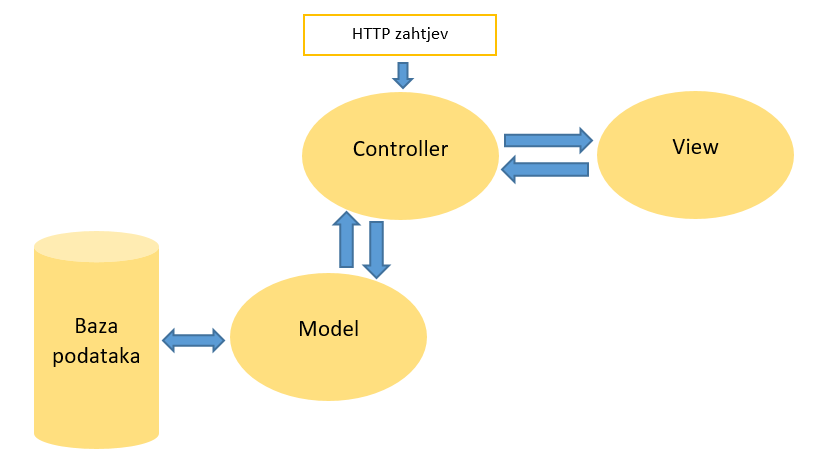
\includegraphics[scale=0.8]{arhitektura/mvc.png} %veličina slike u odnosu na originalnu datoteku i pozicija slike
					\centering
					\caption{Model - View - Controller}
					\label{fig:arhitektura}
		\end{figure}

		\section{Baza podataka}
			
		Za naš projekt odabrali smo \textbf{relacijsku bazu podataka} zbog njezine pogodnosti da prikaže mali dio stvarnog svijeta bez redundancije unutar same baze. Dohvaćanje podataka je relativno brzo i lagano se može paralelizirati. Specifičnu implementaciju relacijske baze podataka koju smo odabrali je \textbf{PostgreSQL}. To je baza podataka otvorenog koda s preko 30 godina aktivnog razvoja zbog kojega je zaslužila svoju čvrstu reputaciju za pouzdanost, bogatstvo opcijama i visokim performansama. Zbog načina na koji je SQL standard napisan, vrlo je slična ostalim SQL bazama podataka.\\ 
		
		Tijekom razvoja koristimo \textbf{H2 bazu}. To je privremena baza podataka koja služi za testiranje koda. Svi zapisi u njoj se nalaze u privremenoj memoriji i nisu perzistentni. Zbog toga je odlična za testiranje. Ona je otvorenog koda, napisana u Javi i ima čvrste sigurnosne postavke. Na nju se možemo povezati s više konekcija i baza podataka je enkriptirana SHA-256 enkripcijom. Ima vrlo malu potrošnju memorije i zauzima relativno malo prostora na disku (oko 2MB). \\ 
		
		Također koristimo \textbf{JPA (Java Persistence API)} koje samo sadrži sučelja za stvaranje Persistence layouta. Dopušta nam da mapiramo entitete tablica i veze između tablica na objekte u Javi. Ovo sučelje definira svoj vlastiti jezik za upite (JPQA). JPQA prevoditelj interpretira kod i piše SQL upite. JPA ne možemo samostalno koristiti, već nam treba konkretna implementacija toga sučelja. Implementacija koju ćemo mi koristiti se zove Hibernate. \\ 
		
		Na bazu podataka se iz Jave spajamo preko \textbf{JdbcTemplatea}. To je snažni mehanizam za spajanje i izvođenje SQL upita. On nam smanjuje količinu koda koju moramo napisati kako bismo izvršavali upite, kao što je spajanje na bazu, kreiranje izraza i zatvaranje konekcija. \\
		\newpage
	Naš model baze podataka sastoji se od sljedećih \textbf{glavnih} i \underline{veznih} tablica:
		\begin{itemize}[noitemsep]
		\item \textbf{user}
		\item \textbf{residence$\_$place}
		\item \textbf{role}
		\item \textbf{mountain$\_$lodge}
		\item \textbf{mountain$\_$path}
		\item \textbf{event}
		\item \textbf{hill}
		\item \textbf{utility}
		\item \textbf{badge}
		\item \textbf{contact$\_$message}
		\item \underline{visit$\_$confirmation}
		\item \underline{friendships}
		\item \underline{frienship$\_$req}
		\item \underline{user$\_$role}
		\item \underline{user$\_$place}
		\item \underline{user$\_$badge}
		\item \underline{mountain$\_$lodge$\_$utility}
		\item \underline{mountain$\_$lodge$\_$report}
		\item \underline{duty$\_$mountaneer}
		\item \underline{event$\_$path}
		\item \underline{event$\_$attendance}
		\item \underline{mountain$\_$path$\_$report}
		\item \underline{mountain$\_$path$\_$grade}
		\item \underline{path$\_$user$\_$wishlist}
		\item \underline{mountain$\_$path$\_$completed}
		\item \underline{badge\_notification}

\end{itemize}
		 \newpage
			\subsection{Opis tablica}
			Primarni ključevi su označeni \textbf{podebljano}, dok su strani ključevi \underline{podvučeni}. \\
			Prikazane su i sve vezne tablice, tako da se nad glavnim tablicama Many-To-Many veze neće navoditi.
			
%Tablice
			\textbf{user} -  ovaj entitet sadrži sve važne informacije o korisniku aplikacije.
			Sadrži atribute: "id", "full$\_$name", "email", "password", "image", "id$\_$place", "date$\_$of$\_$birth" i "description" koji redom predstavljaju jedinstveni identifikacijski broj korisnika, ime i prezime, e-mail korisnika, lozinku korisnika, sliku vidljivu na profilu korisnika, identifikacijski broj mjesta stanovanja korisnika te datum rođenja korisnika.
			Neki podaci o korisniku, kao što su mjesto stanovanja i datum rođenja su opcionalni, i ako ih korisnik ne ispuni njihova vrijednost je \textit{NULL}. Atribut "place\_id" je strani ključ koji referencira entitet \textbf{residence\_place} te se radi o Many-To-One vezi. 
			
			\begin{longtabu} to \textwidth {|X[6, l]|X[6, l]|X[20, l]|}
				\hline \multicolumn{3}{|c|}{\textbf{user - (Korisnik)}}	 \\[3pt] \hline
				\endfirsthead
				
				\hline \multicolumn{3}{|c|}{\textbf{user - (Korisnik)}}	 \\[3pt] \hline
				\endhead
				
				\hline 
				\endlastfoot
				
				\textbf{id} & BIGINT	&  	jedinstveni identifikacijski broj korisnika	\\ \hline
				full$\_$name	& VARCHAR &  ime i prezime korisnika 	\\ \hline 
				email & VARCHAR &  e-mail pomoću kojega se korisnik prijavljuje u sustav \\ \hline 
				password & VARCHAR	&  	lozinka pomoću koje se korisnik prijavljuje u sustav	\\ \hline 
				image & BYTEA	&  	slika vidljiva na profilu korisnika	\\ \hline 
				\underline{place\_id} & BIGINT & strani ključ mjesta stanovanja korisnika iz tablice \textbf{residence\_place}, unos je opcionalan\\ \hline
				date\_of\_birth & DATE & datum rođenja korisnika, unos je opcionalan \\ \hline
				
				
			\end{longtabu}
			\vspace{10mm}
			
			\textbf{residence\_place}  Ovo je entitet koji modelira mjesto stanovanja korisnika. Sadrži atribute: "id" i "name" koji predstavljaju jedinstveni identifikator mjesta te naziv mjesta.
			
			
			\begin{longtabu} to \textwidth {|X[6, l]|X[6, l]|X[20, l]|}
				
				\hline \multicolumn{3}{|c|}{\textbf{residence\_place - (Mjesto stanovanja)}}	 \\[3pt] \hline
				\endfirsthead
				
				\hline \multicolumn{3}{|c|}{\textbf{residence\_place - (Mjesto stanovanja)}}	 \\[3pt] \hline
				\endhead
				
				\hline 
				\endlastfoot
				
				\textbf{id} & BIGINT	&  	jedinstveni indetifikacijski broj mjesta stanovanja	\\ \hline
				name	& VARCHAR &  naziv mjesta 	\\ \hline 
				%\cellcolor{LightBlue} primjer	& VARCHAR &   	\\ \hline 
				
				
			\end{longtabu}
				
				\vspace{10mm}
			\newpage
			\textbf{role} Ovaj entitet modelira ulogu korisnika unutar aplikacije, tzv. "aplikativne role". Određuje razinu ovlasti koje korisnik ima. Sadrži atribute: "id" i "name" koji predstavljaju jedinstveni identifikator uloge te naziv uloge. Dopuštene uloge u našoj aplikaciji su: Planinar, Dežurni planinar i Administrator.
			
			\begin{longtabu} to \textwidth {|X[6, l]|X[6, l]|X[20, l]|}
				
				\hline \multicolumn{3}{|c|}{\textbf{role - (Uloga)}}	 \\[3pt] \hline
				\endfirsthead
				
				\hline \multicolumn{3}{|c|}{\textbf{role - ime tablice}}	 \\[3pt] \hline
				\endhead
				
				\hline 
				\endlastfoot
				
				\textbf{id} & BIGINT	&  jedinstveni ID uloge	\\ \hline
				name	& VARCHAR &  ime uloge 	\\ \hline 
				
			\end{longtabu}
		
		\vspace{10mm}		
		
		\textbf{mountain\_lodge} Ovaj entitet modelira jedan planinarski dom. Sadrži atribute: "id", "name", "image", "elevation" i "hill\_id" koji predstavljaju jedinstveni identifikator planinarskog doma, naziv planinarskog doma, sliku planinarskog doma, nadmorsku visinu te jedinstveni identifikator zemljopisnog područja (visočja) na kojemu se planinarski dom nalazi. Unos slike za neki planinarski dom je opcionalan, a ako se atribut ne popuni njegova vrijednost je \textit{NULL}. Atribut "hill\_id" predstavlja strani ključ koji referencira entitet \textbf{hill} te se radi o Many-To-One vezi. 
		
		\begin{longtabu} to \textwidth {|X[6, l]|X[6, l]|X[20, l]|}
			
			\hline \multicolumn{3}{|c|}{\textbf{mountain\_lodge - (Planinarski dom)}}	 \\[3pt] \hline
			\endfirsthead
			
			\hline \multicolumn{3}{|c|}{\textbf{mountain\_lodge - ime tablice}}	 \\[3pt] \hline
			\endhead
			
			\hline 
			\endlastfoot
			
			\textbf{id} & BIGINT	&  	jedinstveni identifikacijski broj planinarskog doma 	\\ \hline
			name	& VARCHAR &   naziv planinarskog doma	\\ \hline 
			image & BYTEA &  slika planinarskog doma koja se prikazuje unutar aplikacije, unos je opcionalan \\ \hline 
			elevation & INTEGER & nadmorska visina na kojoj se planinarski dom nalazi izražena u kilometrima \\ \hline 
			\underline{hill\_id} & BIGINT	&  strani ključ na tablicu \textbf{hill}, a predstavlja identifikator visočja na kojemu se nalazi planinarski dom	\\ \hline 
			
			
		\end{longtabu}
	\vspace{10mm}		
	
	
	\textbf{utility} Ovaj entitet modelira značajke infrastrukture pojedinog doma. Sadrži atribute "id" i "name" koji predstavljaju jedinstveni identifikacijski broj značajke te naziv značajke. Primjeri takvih značajki su pitka voda, hrana, smještaj, internet.
	
	\newpage
	\begin{longtabu} to \textwidth {|X[6, l]|X[6, l]|X[20, l]|}
		
		\hline \multicolumn{3}{|c|}{\textbf{utility - (Pogodnost, značajka)}}	 \\[3pt] \hline
		\endfirsthead
		
		\hline \multicolumn{3}{|c|}{\textbf{utility - ime tablice}}	 \\[3pt] \hline
		\endhead
		
		\hline 
		\endlastfoot
		
		\textbf{id} & BIGINT	&  jedinstveni identifikator značajke\\ \hline
		name	& VARCHAR &  naziv značajke/pogodnosti \\ \hline 
		
	\end{longtabu}
				\vspace{10mm}		
				
				\textbf{hill} Ovaj entitet modelira pojedino zemljopisno područje, odnosno visočje na kojemu se nalazi pojedini planinarski dom ili planinarska staza. Sadrži atribute: "id" i "name" koji predstavljaju jedinstveni identifikacijski broj visočja te naziv visočja.
				
				\begin{longtabu} to \textwidth {|X[6, l]|X[6, l]|X[20, l]|}
					
					\hline \multicolumn{3}{|c|}{\textbf{hill - (Visočje)}}	 \\[3pt] \hline
					\endfirsthead
					
					\hline \multicolumn{3}{|c|}{\textbf{hill - ime tablice}}	 \\[3pt] \hline
					\endhead
					
					\hline 
					\endlastfoot
					
					\textbf{id} & BIGINT	&  jedinstveni ID visočja 	\\ \hline
					name & VARCHAR	&  ime visočja 	\\ \hline
					
					
				\end{longtabu}
				\vspace{10mm}
			
			\textbf{mountain\_path} Ovaj entitet sadrži informacije o pojedinoj planinarskoj stazi. Sadrži atribute: "id", "name", "start\_point", "end\_point", "avg\_walk\_time", "length", "sea\_level\_diff", "date\_created", "is\_private", "author\_id" i "hill\_id" koji redom predstavljaju jedinstveni identifikacijski broj planinarske staze, naziv staze, polazišnu točku, završnu toku, prosječno vrijeme potrebno da se prepješači staza, duljinu staze, razliku u nadmorskoj visini između početne i završne točke, datum kreiranja pojedine staze od strane korisnika unutar naše aplikacije, vrijednost koja govori je li staza privatna ili javna, korisnika koji je stvorio stazu te identifikator visočja na kojemu se staza nalazi. Atribut "author\_id" te atribut "hill\_id" su strani ključevi obzirom na tablicu \textbf{user} odnosno \textbf{hill} te se radi o Many-To-One vezama.
			
			\begin{longtabu} to \textwidth {|X[6, l]|X[6, l]|X[20, l]|}
				
				\hline \multicolumn{3}{|c|}{\textbf{mountain\_path - (Planinarska staza)}}	 \\[3pt] \hline
				\endfirsthead
				
				\hline \multicolumn{3}{|c|}{\textbf{mountain\_path - (Planinarska staza)}}	 \\[3pt] \hline
				\endhead
				
				\hline 
				\endlastfoot
				
				\textbf{id} & BIGINT	& jedinstveni identifikacijski broj planinarske staze	\\ \hline
				name	& VARCHAR &  naziv staze	\\ \hline 
				start\_point & VARCHAR & naziv početne točke staze  \\ \hline 
				end\_point & VARCHAR &  naziv završne točke staze \\ \hline 
				avg\_walk\_time & TIME &  prosječno vrijeme potrebno za prepješačiti stazu\\ \hline 
				length & INTEGER & duljina staze u metrima\\ \hline 
				sea\_level\_diff & INTEGER & razlika u nadmorskoj visini između početne i završne točke staze\\ \hline 
				date\_created & DATE &  datum stvaranja staze unutar aplikacije\\ \hline 
				is\_private & BOOLEAN	&  atribut koji govori je li korisnik stazu stvara privatno ili javno  \\ \hline 
				\underline{author\_id} & BIGINT	&  	identifikacijski broj korisnika koji je stvorio stazu unutar aplikacije\\ \hline 
				\underline{hill\_id} & BIGINT	&  identifikacijski broj visočja na kojemu se staza nalazi\\ \hline 
				
				
			\end{longtabu}
			\vspace{10mm}
			
			\textbf{event} Ovaj entite modelira jedan događaj koji stvara korisnik unutar naše aplikacije. Jedan događaj počinje u određeno vrijeme "start\_date", te završava u određeno vrijeme: "end\_date". Svaki događaj, odnosno planinarski izlet sastoji se od jedne ili više planinarskih staza koje se obilaze tijekom tog planinarskog izleta. Osim toga, planinarski izlet ima svoj opis: "description", gdje korisnik može reći više pojedinosti o samom planinarskom izletu. Osim toga, ovaj entitet sadrži atribute: "id", "name", "date\_created" i "author\_id" koji predstavljaju jedinstveni identifikacijski broj događaja, naziv događaja, vrijeme kada je korisnik stvorio događaj unutar aplikacije te jedinstveni identifikacijski broj korisnika koji je stvorio događaj. Atribut "author\_id" je strani ključ koji se odnosi na tablicu \textbf{user} te se radi o Many-To-One vezi.
			
			\begin{longtabu} to \textwidth {|X[6, l]|X[6, l]|X[20, l]|}
				
				\hline \multicolumn{3}{|c|}{\textbf{event - (Planinarski događaj)}}	 \\[3pt] \hline
				\endfirsthead
				
				\hline \multicolumn{3}{|c|}{\textbf{event - (Planinarski događaj)}}	 \\[3pt] \hline
				\endhead
				
				\hline 
				\endlastfoot
				
				\textbf{id} & BIGINT	&  	jedinstveni identifikacijski broj planinarskog izleta 	\\ \hline
				name	& VARCHAR & naziv događaja 	\\ \hline 
				description & VARCHAR &  pojedinosti vezane uz događaj \\ \hline 
				start\_date & TIMESTAMP	&  vrijeme i datum početka planinarskog izleta	\\ \hline 
				end\_date & TIMESTAMP	&  	vrijeme i datum završetka planinarskog izleta	\\ \hline 
				date\_created & TIMESTAMP	&  vrijeme i datum stvaranja izleta unutar aplikacije\\ \hline 
				\underline{author\_id} & BIGINT	& jedinstveni identifikacijski broj korisnika koji je stvorio događaj unutar aplikacije		\\ \hline 
				
				
			\end{longtabu}
			\vspace{10mm}
			
			\textbf{badge} Ovaj entitet modelira jedan bedž, odnosno priznanje koje korisnik može zaslužiti kao planinar. Korisnik priznanja zaslužuje za svoju aktivnost koja se gleda na osnovu arhive planinarskih domova i staza, te se uzimaju u obzir značajke kao što su: broj posjećenih planinarskih domova, broj odrađenih planinarskih staza i sl. Entitet sadrži atribute "id" i "name" koji predstavljaju jedinstveni identifikacijski broj priznanja te naziv priznanja.
			
			\begin{longtabu} to \textwidth {|X[6, l]|X[6, l]|X[20, l]|}
				
				\hline \multicolumn{3}{|c|}{\textbf{badge - (Priznanje)}}	 \\[3pt] \hline
				\endfirsthead
				
				\hline \multicolumn{3}{|c|}{\textbf{badge - (Priznanje)}}	 \\[3pt] \hline
				\endhead
				
				\hline 
				\endlastfoot
				
				\textbf{id}	& BIGINT &   jedinstveni identifikacijski broj priznanja	\\ \hline 
				name & VARCHAR &  naziv priznanja \\ \hline 
				
				
			\end{longtabu}
		
				\vspace{10mm}
				
				\textbf{contact\_message} Ovaj entitet modelira poruke koje korisnik može slati administratoru u slučaju npr. otvaranja novog planinarskog doma. Sadrži atribute: "id", "description", "date\_send" koji redom predstavljaju jedinstveni identifikacijski broj poruke, opis odnosno sadržaj poruke te datum i vrijeme slanja poruke.
				
				\begin{longtabu} to \textwidth {|X[6, l]|X[6, l]|X[20, l]|}
					
					\hline \multicolumn{3}{|c|}{\textbf{contact\_message - (Poruke administratoru)}}	 \\[3pt] \hline
					\endfirsthead
					
					\hline \multicolumn{3}{|c|}{\textbf{badge - (Priznanje)}}	 \\[3pt] \hline
					\endhead
					
					\hline 
					\endlastfoot
					
					\textbf{id}	& BIGINT &   jedinstveni identifikacijski broj poruke	\\ \hline 
					description & VARCHAR &  sadržaj poruke \\ \hline 
					created\_on & DATE &  datum i vrijeme slanja poruke \\ \hline 
					\underline{user\_id} & BIGINT	& jedinstveni identifikacijski broj korisnika koji je stvorio poruku unutar aplikacije		\\ \hline 
					
				\end{longtabu}
				\vspace{10mm}
				
				
				
				\textbf{visit\_confirmation} Ovo je vezna tablica koja nam modelira zahtjeve koje korisnik šalje dežurnim planinarima kada je posjetio određeni dom. Tablica predstavlja Many-To-Many vezu između entiteta \textbf{user} i entiteta \textbf{mountain\_lodge}. Osim stranih ključeva "user\_id" i "lodge\_id" sadrži i atribute "time\_requested" i "status" koji redom predstavljaju vrijeme slanja zahtjeva te status obrade zahtjeva za posjetom, koji može biti: ACCEPTED (Prihvaćen), REJECTED (Odbijen) ili PENDING (aktivan).
				
				\begin{longtabu} to \textwidth {|X[6, l]|X[6, l]|X[20, l]|}
					
					\hline \multicolumn{3}{|c|}{\textbf{visit\_confirmation - (Zahtjev za potvrdom posjeta)}}	 \\[3pt] \hline
					\endfirsthead
				
					\hline 
					\endlastfoot
					
					\underline{user\_id} & BIGINT	&  strani ključ korisnika koji traži potvrdu posjeta iz tablice \textbf{user}\\ \hline
					\underline{lodge\_id}	& BIGINT & strani ključ planinarskog doma kojeg posjećuje iz tablice \textbf{mountain\_lodge} 	\\ \hline 
					time\_requested & TIMESTAMP &  datum i vrijeme slanja zahtjeva za posjetom \\ \hline 
					status & VARCHAR	&  status zahtjeva	\\ \hline  
		
		\end{longtabu}
		\vspace{10mm}
	
			\textbf{friendships} Ovo je vezna tablica koja sadrži Many-To-Many vezu između dva korisnika, a služi nam za modeliranje prijateljstava, odnosno pripadanja istoj planinarskoj zajednici. Sadrži atribute "user\_id1" i "user\_id2" koji predstavljaju strane ključeve na tablicu \textbf{user} i govore nam tko su korisnici koji pripadaju istoj zajednici, te atribut "friendship\_created" koji nam govori o datumu i vremenu stvaranja prijateljstva.
			
			\begin{longtabu} to \textwidth {|X[6, l]|X[6, l]|X[20, l]|}
				
				\hline \multicolumn{3}{|c|}{\textbf{friendships - (Prijatelji)}}	 \\[3pt] \hline
				\endfirsthead
				
				\hline \multicolumn{3}{|c|}{\textbf{friendships - (Prijatelji)}}	 \\[3pt] \hline
				\endhead
				
				\hline 
				\endlastfoot
				
				\underline{user\_id1} & BIGINT	&  strani ključ koji se odnosi na jednog korisnika člana veze "prijatelji"	\\ \hline
				\underline{user\_id2}	& BIGINT &   strani ključ koji se odnosi na drugog korisnika člana veze "prijatelji"\\ \hline 
				friendship$\_$ \text{created}	& TIMESTAMP &   vrijeme i datum kada su dva određena dva korisnika postala prijatelji	\\ \hline 
				%\cellcolor{LightBlue} primjer	& VARCHAR &   	\\ \hline 
				
				
			\end{longtabu}
			\vspace{10mm}

			\textbf{friendship\_req} Ovaj entitet sadrži informaciju o poslanom zahtjevu za prijateljstvo između 2 korisnika. Sadrži atribute: "friendship\_send" te "friendship\_recieve" koji su oba strani ključevi iz tablice \textbf{user}, a predstavljaju identifikacijski broj pošiljatelja te primatelja zahtjeva za prijateljstvo. Radi se o refleksivnoj Many-to-Many vezi.
			
			\begin{longtabu} to \textwidth {|X[6, l]|X[6, l]|X[20, l]|}
				
					\hline \multicolumn{3}{|c|}{\textbf{friendship\_req - (Zahtjevi za prijateljstvom)}}	 \\[3pt] \hline
				\endfirsthead
				
				\hline \multicolumn{3}{|c|}{\textbf{friendship\_req - (Zahtjevi za prijateljstvom)}}	 \\[3pt] \hline
				\endhead
				
				\hline 
				\endlastfoot
				
				\underline{friendship\_} \underline{send} & BIGINT	&  strani ključ korisnika koji šalje zahtjev za prijateljstvom iz tablice \textbf{user} 	\\ \hline
				\underline{friendship\_} \underline{recieve}	& BIGINT &   strani ključ korisnika koji prima zahtjev za prijateljstvom	iz tablice \textbf{user}\\ \hline 
				%\cellcolor{LightBlue} primjer	& VARCHAR &   	\\ \hline 
				
				
			\end{longtabu}
		\vspace{10mm}
		
		\textbf{user\_role} Vezna tablica koja modelira Many-to-Many vezu između entiteta \textbf{user} i entiteta \textbf{role}. Jedan korisnik može imati više uloga, dok jednu ulogu može imati više različitih korisnika. Sadrži atribute "role\_id" te "user\_id" koji redom predstavljaju identifikacijski broj uloge te identifikacijski broj korisinika.
		
		\begin{longtabu} to \textwidth {|X[6, l]|X[6, l]|X[20, l]|}
			
			\hline \multicolumn{3}{|c|}{\textbf{user\_role}}	 \\[3pt] \hline
			\endfirsthead
			
			\hline \multicolumn{3}{|c|}{\textbf{user\_role}}	 \\[3pt] \hline
			\endhead
			
			\hline 
			\endlastfoot
			
			\underline{user\_id} & BIGINT	&  	strani ključ korisnika iz entiteta \textbf{user}	\\ \hline
			\underline{role\_id}	& BIGINT &  strani ključ uloge, odnosno aplikativne role iz entiteta \textbf{role}\\ \hline 
			
			
		\end{longtabu}
			\vspace{10mm}
			
			\textbf{user\_badge} Ovaj entitet sadrži informaciju o Many-To-Many odnosu između bedževa (priznanja) i korisnika. Sadrži atribute: "user\_id", "badge\_id" i "date\_recieved" koji redom predstavljaju identifikacijski broj korisnika, identifikacijski broj priznanja te vrijeme dobivanja priznanja.
			
			\begin{longtabu} to \textwidth {|X[6, l]|X[6, l]|X[20, l]|}
				
				\hline \multicolumn{3}{|c|}{\textbf{user\_badge}}	 \\[3pt] \hline
				\endfirsthead
				
				\hline \multicolumn{3}{|c|}{\textbf{user\_badge}}	 \\[3pt] \hline
				\endhead
				
				\hline 
				\endlastfoot
				
				\underline{user\_id} & BIGINT	&  strani ključ korisnika kojemu je pripisan pojedini bedž iz tablice \textbf{user}\\ \hline
				\underline{badge\_id}	& BIGINT &  strani ključ bedža kojega je dobio pojedini korisnik iz tablice \textbf{badge}	\\ \hline 
				date\_recieved & DATE & datum dobivanja pojedinog bedža za određenog korisnika  \\ \hline 
				
				
			\end{longtabu}
			\vspace{10mm}

			\textbf{event\_attendance} Modelira Many-To-Many vezu između korisnika i događaja (planinarskog izleta) na kojemu korisnik želi sudjelovati. Sadrži atribute "user\_id" te "event\_id" koji predstavljaju jedinstveni identifikator korisnika koji sudjeluje na događaju te jedinstveni identifikator događaja.
			
			\begin{longtabu} to \textwidth {|X[6, l]|X[6, l]|X[20, l]|}
				
				\hline \multicolumn{3}{|c|}{\textbf{event\_attendance}}	 \\[3pt] \hline
				\endfirsthead
				
				\hline \multicolumn{3}{|c|}{\textbf{event\_attendance}}	 \\[3pt] \hline
				\endhead
				
				\hline 
				\endlastfoot
				
				\underline{user\_id} & BIGINT	&  	strani ključ korisnika koji će prisustvovati događaju iz tablice \textbf{user}	\\ \hline
				\underline{event\_id}	& BIGINT &  strani ključ događaja kojemu određena osoba pristupa iz tablice \textbf{event}\\ \hline 
				
				
			\end{longtabu}
			\vspace{10mm}		
			
			\textbf{event\_path} Ovaj entitet sadrži informaciju o Many-To-Many vezi između planinarske staze i nekog planinarskog događaja. Sadrži atribute: "path\_id" te "event\_id" koji predstavljaju identifikacijski broj planinarske staze i identifikacijski broj nekog planinarskog događaja. Osim toga, sadrži atribut "event\_day" koji nam govori o rednom broju dana tijekom kojega se na određenom planinarskom događaju odrađuje određena planinarska staza.
			
			\begin{longtabu} to \textwidth {|X[6, l]|X[6, l]|X[20, l]|}
				
				\hline \multicolumn{3}{|c|}{\textbf{event\_path}}	 \\[3pt] \hline
				\endfirsthead
				
				\hline \multicolumn{3}{|c|}{\textbf{event\_path}}	 \\[3pt] \hline
				\endhead
				
				\hline 
				\endlastfoot
				
				\underline{path\_id} & BIGINT	&  	strani ključ staze koja je dio nekog događaja iz tablice \textbf{mountain\_path}	\\ \hline
				\underline{event\_id}	& BIGINT &  strani ključ događaja u kojemu se pojedina staza odrađuje, iz tablice \textbf{event}	\\ \hline 
				event\_day	& INTEGER &  redni broj dana kojega se unutar jednog događaja obilazi određena staza	\\ \hline 
				
			\end{longtabu}
			\vspace{10mm}
		
			\textbf{badge\_notification} Ovaj entitet sadrži informaciju o Many-To-Many odnosu između bedževa i korisnika, ali samo u smislu obavijesti korisniku. Kada korisnik potvrdi da je primio obavijest, pojedini unos se briše iz ovog entiteta. Sadrži atribute: "user\_id" te "badge\_id" koji predstavljaju identifikator korisnika koji je dobio priznanje čiji je identifikator "badge\_id".
			
			\begin{longtabu} to \textwidth {|X[6, l]|X[6, l]|X[20, l]|}
				
				\hline \multicolumn{3}{|c|}{\textbf{badge\_notification}}	 \\[3pt] \hline
				\endfirsthead
				
				\hline \multicolumn{3}{|c|}{\textbf{badge\_notification}}	 \\[3pt] \hline
				\endhead
				
				\hline 
				\endlastfoot
				
				\underline{user\_id} & BIGINT	&  strani ključ korisnika kojemu je pripisan pojedini bedž iz tablice \textbf{user}\\ \hline
				\underline{badge\_id}	& BIGINT) &  strani ključ bedža kojega je dobio pojedini korisnik iz tablice \textbf{badge}\\ \hline  
				
				
			\end{longtabu}
			\vspace{10mm}		
		
			\textbf{mountain\_lodge\_utility} Vezna tablica koja modelira Many-to-Many vezu između planinarskih domova i infrastrukturnih značajki koje ti domovi posjeduju. Sadrži atribute "lodge\_id" te "utility\_id" koji predstavljaju identifiaktor planinarskog doma te identifikator odgovarajuće značajke.
			
			\begin{longtabu} to \textwidth {|X[6, l]|X[6, l]|X[20, l]|}
				
				\hline \multicolumn{3}{|c|}{\textbf{mountain\_lodge\_utility}}	 \\[3pt] \hline
				\endfirsthead
				
				\hline \multicolumn{3}{|c|}{\textbf{mountain\_lodge\_utility}}	 \\[3pt] \hline
				\endhead
				
				\hline 
				\endlastfoot
				
				\underline{lodge\_id} & BIGINT	&  strani ključ kojemu je pripisan pojedini planinarski dom iz tablice  \textbf{mountain\_lodge}\\ \hline
				\underline{utility\_id}	& BIGINT &  strani ključ kojemu je pripisana pojedina značajka iz tablice \textbf{utility} \\ \hline 
				
				
			\end{longtabu}
			\vspace{10mm}
			
			\textbf{mountain\_path\_grade} Vezna tablica koja nam govori o ocjenama koje pojedini korisnik dodjeljuje pojedinoj planinarskoj stazi. Radi se o Many-To-Many veznoj tablici. Sadrži atribute "user\_id", "path\_id" te "grade", koji redom predstavljaju identifikacijski broj korisnika, identifikacijski broj planinarske staze te ocjenu koju je taj korisnik dodijelio toj stazi.
			
			\begin{longtabu} to \textwidth {|X[6, l]|X[6, l]|X[20, l]|}
				
				\hline \multicolumn{3}{|c|}{\textbf{mountain\_path\_grade}}	 \\[3pt] \hline
				\endfirsthead
				
				\hline \multicolumn{3}{|c|}{\textbf{mountain\_path\_grade}}	 \\[3pt] \hline
				\endhead
				
				\hline 
				\endlastfoot
				
				\underline{user\_id} & BIGINT	& strani ključ korisnika koji daje ocjenu iz tablice \textbf{user}  	\\ \hline
				\underline{path\_id}	& BIGINT &   strani ključ planinarske staze koja se ocjenjuje iz tablice \textbf{mountain\_path}	\\ \hline 
				grade & INTEGER & ocjenu koju je korisnik dodijelio za konkretnu stazu  \\ \hline 
				
				
			\end{longtabu}
			\vspace{10mm}		
		
			\textbf{path\_user\_wishlist} Vezna tablica koja modelira željene planinarske staze za pojedinog korisnika. To su staze koje korisnik ima namjeru prepješačiti, ali još nije uspio. Sadrži atribute "user\_id" i "path\_id" koji predstavljaju identifikator korisnika te identifikator staze koju korisnik želi prepješačiti.
		
			\begin{longtabu} to \textwidth {|X[6, l]|X[6, l]|X[20, l]|}
				
				\hline \multicolumn{3}{|c|}{\textbf{path\_user\_wishlist}}	 \\[3pt] \hline
				\endfirsthead
				
				\hline \multicolumn{3}{|c|}{\textbf{path\_user\_wishlist}}	 \\[3pt] \hline
				\endhead
				
				\hline 
				\endlastfoot
				
				\underline{user\_id} & BIGINT	& strani ključ korisnika  koji želi prepješačiti neku stazu iz tablice \textbf{user}	\\ \hline
				\underline{path\_id} & BIGINT	& strani ključ staze koju korisnik želi prepješačiti iz tablice \textbf{mountain\_path}	\\ \hline
				
				
			\end{longtabu}
			\vspace{10mm}			
			
			\textbf{mountain\_path\_completed} Ovaj entitet sadrži informaciju o Many-To-Many odnosu između pojedinog korisnika i staza koje je već prepješačio, odnosno ovaj entitet modelira arhivu staza.
			
			\begin{longtabu} to \textwidth {|X[6, l]|X[6, l]|X[20, l]|}
				
				\hline \multicolumn{3}{|c|}{\textbf{mountain\_path\_completed}}	 \\[3pt] \hline
				\endfirsthead
				
				\hline \multicolumn{3}{|c|}{\textbf{mountain\_path\_completed}}	 \\[3pt] \hline
				\endhead
				
				\hline 
				\endlastfoot
				
				\underline{user\_id} & BIGINT	& strani ključ korisnika  koji je prepješačio pojedinu stazu iz tablice \textbf{user}	\\ \hline
				path\_id	& BIGINT &   strani ključ staze koju je konkretni korisnik prepješačio iz tablice \textbf{mountain\_path}	\\ \hline 
				date\_completed & DATE & datum kojega je određeni korisnik prepješačio određenu stazu  \\ \hline 
				
				
			\end{longtabu}
			\vspace{10mm}
		
			\textbf{mountain\_path\_report} Vezna tablica koja modelira prijavu netočnih ili nepreciznih informacija vezanih uz pojedinu plainarsku stazu. Korisnik kojemu je identifikacijski broj "user\_id" prijavljuje netočne informacije vezane uz planinarsku stazu identifikatora "path\_id", a osim toga bilježi se i vrijeme prijave pogreške kao atribut "date\_report", opis pogreške kao atribut "description" te status pogreške kao atribut "status" koji označava je li administrator pogrešku prihvatio, odbio ili je ona i dalje aktivna.
			\begin{longtabu} to \textwidth {|X[6, l]|X[6, l]|X[20, l]|}
				
				\hline \multicolumn{3}{|c|}{\textbf{mountain\_path\_report}}	 \\[3pt] \hline
				\endfirsthead
				
				\hline \multicolumn{3}{|c|}{\textbf{mountain\_path\_report}}	 \\[3pt] \hline
				\endhead
				
				\hline 
				\endlastfoot
				
				\underline{user\_id} & BIGINT	& strani ključ korisnika  koji prijavljuje netočnu ili nepreciznu informaciju vezanu uz neku planinarsku stazu, a odnosi se na tablicu \textbf{user}	\\ \hline
				\underline{path\_id}	& BIGINT &   strani ključ planinarske staze koju korisnik prijavljuje, a odnosi se na tablicu \textbf{mountain\_path}	\\ \hline 
				description & VARCHAR & opsi netočne ili neprecizne informacije o nekoj stazi  \\ \hline 
				status & VARCHAR & status prijavljene pogreške  \\ \hline
				date\_report & TIMESTAMP & vrijeme i datum prijave pogreške vezane uz određenu planinarsku stazu  \\ \hline
				
		
				
				
			\end{longtabu}
					\vspace{10mm}
		
		\textbf{mountain\_lodge\_report} Vezna tablica koja modelira prijavu netočnih ili nepreciznih informacija vezanih uz pojedini plainarski dom. Korisnik kojemu je identifikacijski broj "user\_id" prijavljuje netočne informacije vezane uz planinarski dom identifikatora "lodge\_id", a osim toga bilježi se i vrijeme prijave pogreške kao atribut "date\_report", opis pogreške kao atribut "description" te status pogreške kao atribut "status" koji označava je li administrator pogrešku prihvatio, odbio ili je ona i dalje aktivna.
		\begin{longtabu} to \textwidth {|X[6, l]|X[6, l]|X[20, l]|}
			
			\hline \multicolumn{3}{|c|}{\textbf{mountain\_lodge\_report}}	 \\[3pt] \hline
			\endfirsthead
			
			\hline \multicolumn{3}{|c|}{\textbf{mountain\_lodge\_report}}	 \\[3pt] \hline
			\endhead
			
			\hline 
			\endlastfoot
			
			\underline{user\_id} & BIGINT	& strani ključ korisnika  koji prijavljuje netočnu ili nepreciznu informaciju vezanu uz neki planinarski dom, a odnosi se na tablicu \textbf{user}	\\ \hline
			\underline{lodge\_id}	& BIGINT &   strani ključ planinarskog doma koji korisnik prijavljuje, a odnosi se na tablicu \textbf{mountain\_lodge}	\\ \hline 
			description & VARCHAR & opsi netočne ili neprecizne informacije o nekom planinarskom domu  \\ \hline 
			status & VARCHAR & status prijavljene pogreške  \\ \hline
			date\_report & VARCHAR & vrijeme i datum prijave pogreške vezane uz određeni planinarski dom  \\ \hline
			
			
			
			
		\end{longtabu}
			\vspace{10mm}
		
			\textbf{duty\_mountaneer} Vezna tablica koja modelira Many-To-Many vezu između planinarskog doma identifikatora "lodge\_id" i planinara identifikatora "user\_id", koji je dežurni planinar za taj dom.
			
			\begin{longtabu} to \textwidth {|X[6, l]|X[6, l]|X[20, l]|}
				
				\hline \multicolumn{3}{|c|}{\textbf{duty\_mountaneer}}	 \\[3pt] \hline
				\endfirsthead
				
				\hline \multicolumn{3}{|c|}{\textbf{duty\_mountaneer}}	 \\[3pt] \hline
				\endhead
				
				\hline 
				\endlastfoot
				
				\underline{user\_id} & BIGINT	& strani ključ korisnika koji je dežurni planinar iz tablice \textbf{user}	\\ \hline
				\underline{lodge\_id}	& BIGINT &   strani ključ planinarskog doma u kojemu je planinar dežuran iz tablice \textbf{mountain\_lodge}	\\ \hline 
				
				
			\end{longtabu}
			\vspace{10mm}



			\subsection{Dijagram baze podataka}
				
				\begin{figure}[H]
					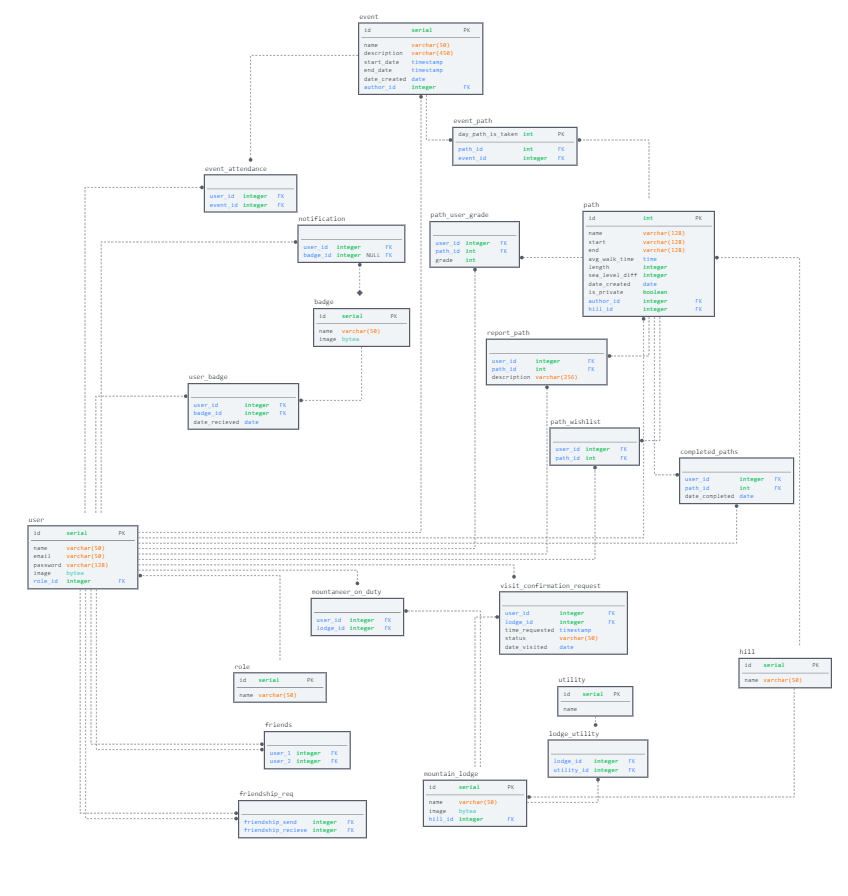
\includegraphics[scale=0.4, height=180mm]{slike/database.png} %veličina slike u odnosu na originalnu datoteku i pozicija slike
					\centering
					\caption{Dijgram baze podataka}
					\label{fig:slične aplikacije}
				\end{figure}
			
			\eject
			
			
		\section{Dijagram razreda}
		
			\textit{Potrebno je priložiti dijagram razreda s pripadajućim opisom. Zbog preglednosti je moguće dijagram razlomiti na više njih, ali moraju biti grupirani prema sličnim razinama apstrakcije i srodnim funkcionalnostima.}\\
			
			\textbf{\textit{dio 1. revizije}}\\
			
			\textit{Prilikom prve predaje projekta, potrebno je priložiti potpuno razrađen dijagram razreda vezan uz \textbf{generičku funkcionalnost} sustava. Ostale funkcionalnosti trebaju biti idejno razrađene u dijagramu sa sljedećim komponentama: nazivi razreda, nazivi metoda i vrste pristupa metodama (npr. javni, zaštićeni), nazivi atributa razreda, veze i odnosi između razreda.}\\
			
			\textbf{\textit{dio 2. revizije}}\\			
			
			\textit{Prilikom druge predaje projekta dijagram razreda i opisi moraju odgovarati stvarnom stanju implementacije}
			
			
			
			\eject
		
		%\section{Dijagram stanja}
			
			
		%	\textbf{\textit{dio 2. revizije}}\\
		%	
		%	\textit{Potrebno je priložiti dijagram stanja i opisati ga. Dovoljan je jedan dijagram stanja koji prikazuje \textbf{značajan dio funkcionalnosti} sustava. Na primjer, stanja korisničkog sučelja i tijek korištenja neke ključne funkcionalnosti jesu značajan dio sustava, a registracija i prijava nisu. }
			
			
		%	\eject 
		
		%\section{Dijagram aktivnosti}
		%	
		%	\textbf{\textit{dio 2. revizije}}\\
			
		%	 \textit{Potrebno je priložiti dijagram aktivnosti s pripadajućim opisom. Dijagram aktivnosti treba prikazivati značajan dio sustava.}
			
		%	\eject
		%\section{Dijagram komponenti}
		
		%	\textbf{\textit{dio 2. revizije}}\\
		
		%	 \textit{Potrebno je priložiti dijagram komponenti s pripadajućim opisom. Dijagram komponenti treba prikazivati strukturu cijele aplikacije.}